%-----------------------------------------------------------------------
\subsection{Mode and Level}
%-----------------------------------------------------------------------
%\tbc
%Marielle Petit


The "Management of Modes and Levels" function is mainly described in chapter 4
and 5 of \citep{subset-026}. Modes and levels define the status of the ETCS
regarding on-board functional status and track infrastructure.

\begin{landscape}
\begin{figure}[hbtp]
\centering
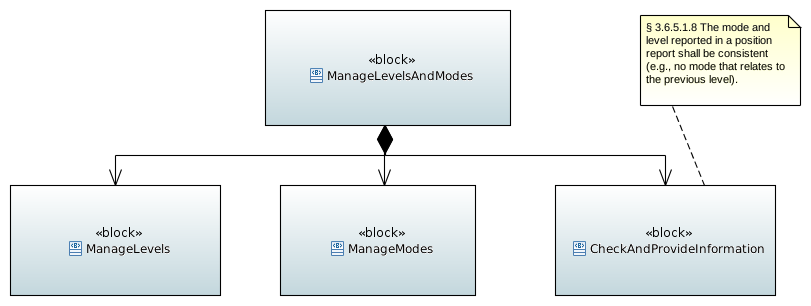
\includegraphics[scale=1]{../SysML/FunctionalArchitecture.png}
\caption{High level Architecture}
\end{figure}
\end{landscape}

\subsubsection{Function Level Management}%Mainfunction receive track data. Name should be be defined and substituded by the designer of the function.
\paragraph{Reference to the SRS or other Requirements}

see \citep{subset-026} section 5.10

\paragraph{Short description of the functionality}

The level management subsystem receives level transition order tables and selects the order with the highest probability. It stores the information about the selected transition order and transits to the requested level once the train passes the location of the level transition.

If required, the driver is asked to acknowledge the transition, in case of no acknowledge or if conditions for the level transition are not fulfilled, the train gets tripped.

\paragraph{Interface}

The interface consists of the following inputs:

\begin{itemize}
\item \emph{conditional transitions:} a priority table containing the
  conditional level transition orders (from paquet 46)
\item \emph{level transition priority table:} a priority table containing the
  (non-conditional) level transition orders (from paquet 41)
\item \emph{train standstill:} a Boolean value indicating whether the train is
  at standstill (from odometry)
\item \emph{driver level transition:} a level transition order selected by the
  driver (from DMI)
\item \emph{ERTMS capabilities:} the ERTMS capabilities of the track
\item \emph{getAck:} Boolean input that signals the acknowledgment of the
  driver (from DMI)
\item \emph{resetIdle:} Boolean input to reset without acknowledge
\item \emph{currentDistance:} the current position of the train given with the
  same reference as the position of the level transition order (train position , from localisation)
\item \emph{ackDistance:} the maximal distance for driver acknowledge after
  the level transition (from paquet 41)
\item \emph{immediateAck:} a Boolean that signals that an immediate acknowledge
  is required
\item \emph{received L2 L3 MA:} a Boolean that indicates that a level 2 or level
  3 movement authority for the track behind the level transition has been
  received (from paquet 15)
\item \emph{received L1 MA:} a Boolean that indicates that a level 1 movement
  authority for the track behind the level transition has been received (from paquet 12)
\item \emph{received target speed:} a Boolean indicating that a target speed for
  the track behind the level transition has been received (from paquet 27) ?
\end{itemize}

and the following outputs:

\begin{itemize}
\item \emph{next level:} the next level after this computation cycle
\item \emph{Trip train:} a Boolean indicating whether the train should be
  tripped
\item \emph{previous level:} the previous level before this computation cycle
\item \emph{needsAckFromDriver:} a Boolean that indicates whether an
  acknowledgment from the driver is necessary
\end{itemize}

\paragraph{Functional Design Description}

On the most abstract level the design consists of the \emph{manage\_priorities} function which takes the level transition order priority tables as inputs and computes the highest priority transition.

This transition order is the fed to the \emph{computeLevelTransitions} operator. This operator consists of three main parts. The \emph{ComputeTransitionConditions} operator that emits the fulfilled conditions to change from a given level to a new level, the \emph{LevelStateMachine} that stores the current level and takes the computed change conditions as input for possible level transitions and finally the \emph{driverAck} operator which contains a state machine that stores the information whether the system is currently waiting for a driver acknowledge and emits the train trip information if necessary.


\paragraph{Reference to the Scade Model}

The Scade model is available on github:
\url{https://github.com/openETCS/modeling/tree/master/openETCS ArchitectureAndDesign/Work Groups/Group 3/SCADE/LevelManagement/}

%%%%%%%%%%%%%%%%%%%%%%%%%%%%%%%%%%%%%%%%%%%%%%%%%%%%

\subsubsection{Function Mode Management}%Mainfunction receive track data. Name should be be defined and substituded by the designer of the function.
\paragraph{Reference to the SRS or other Requirements}
see \citep{subset-026} sections 4.4, 4.6, 5.4, 5.5, 5.6, 5.7, 5.8, 5.9, 5.11, 5.12, 5.13, 5.19

\paragraph{Short description of the functionality}


This function is in charge of the computation of new mode to apply according to conditions from inputs (track information, driver interactions, train data,...) and other functions.

\paragraph{Interface}

The inputs are the following:
\begin{itemize}
\item \emph{Cab} identification of the current cabin (A or B)
\item \emph{Continue\_shunting\_Function\_Active}: boolean to describe the activation state of the shunting function
\item \emph{Current\_Level}: outputs of the Level management function
\item \emph{Data\_From\_DMI}: set of data received from the driver via the DMI interface, indeed:
\begin{itemize}
\item \emph{Ack\_LS : bool} Driver acknoledges LS mode
\item \emph{Ack\_OS : bool}
\item \emph{Ack\_RV : bool}
\item \emph{Ack\_SH : bool}
\item \emph{Ack\_SN : bool}
\item \emph{Ack\_SR : bool}
\item \emph{Ack\_TR : bool}
\item \emph{Ack\_UN : bool}
\item \emph{Req\_Exit\_SH : bool} driver selects exit of shunting
\item \emph{Req\_NL : bool} Driver requests NL mode
\item \emph{Req\_Override : bool} Driver requests override function
\item \emph{Req\_SH : bool} driver requests SH mode
\item \emph{Req\_Start : bool} Driver requests start of mission
\item \emph{ETCS\_Isolated: bool}: isolation status of the ETCS
\end{itemize}
\item \emph{Data\_From\_Localisstion}: set of data received from the function in charge of localistion of the train, indeed:
\begin{itemize}
\item \emph{BG\_In\_List\_Expected\_BG\_In\_SR : bool}: the identity of the overpass balise group is in the list of expected balises related to SR mode (from SR to trip mode condition 36)
\item \emph{BG\_In\_List\_Expected\_BG\_In\_SH : bool}: the identity of the overpass balise group is in the list of expected balises related to SH mode (from SH to trip mode condition 52)
\item \emph{Linked\_BG\_In\_Wrong\_Direction : bool} balise group contained in the linking information is passed in the unexpected direction (from FS, LS, OS to trip mode condition 66) \emph{Localisaion function ?}
\item \emph{Train\_Position}: output provided by function in charge of computation of train possition (type	TrainPosition\_Types\_Pck::trainPosition\_T)	\item \emph{Train\_Speed : Obu\_BasicTypes\_Pkg::Speed\_T} provided by odometry function
\item \emph{Train\_Standstill : bool} provided by odometry function
\end{itemize}
\item \emph{Data\_From\_Speed\_and\_Supervision}: set of data received from the function in charge of speed and supervision management, indeed:
\begin{itemize}
\item \emph{Estim\_front\_End\_overpass\_SR\_Dist : bool}: the train overpass the SR distance with its estimated front end (from SR to trip mode condition 42) 
\item \emph{Estim\_Front\_End\_Rear\_SSP : bool}: estimated front end is rear of the start location of either SSP or gradient profile stored on-board (from FS, LS, OS to trip mode condition 69)
\item \emph{Override\_Function\_Active}: boolean to indicate the state of the activation function 	  	
\item \emph{EOA\_Antenna\_Overpass : bool}: the train overpasses the  EOA  with min safe antenna position Level 1 (from FS, LS, OS to trip mode condition 12)
\item \emph{EOA\_Front\_End : bool} the train overpasses the  EOA  with min safe front end, Level 2 or 3 (from FS, LS, OS to trip mode condition 16)
\item \emph{Train\_Speed\_Under\_Overide\_Limit : bool} supervision when override function is active (to SR mode condition 37)
\end{itemize}
\item \emph{Data\_From\_TIU : TIU\_Types\_Pkg::Message\_Train\_Interface\_to\_EVC\_T}:message provided by TIU interface
\item \emph{Data\_From\_Track}: set of data received from track side (via RBC or Balises telegram), indeed:
\begin{itemize}
\item \emph{MA\_SSP\_Gradiant\_Available : bool} MA, SSP and gradient have been received, checked and stored on-board from paquet 12, 15, 21 and 27 or message 3 or 33
\item \emph{Mode\_Profile\_On\_Board : Level\_And\_Mode\_Types\_Pkg::T\_Mode\_Profile} from packet 80
\item \emph{Shunting\_granted\_By\_RBC : bool} from message 27 and 28
\item \emph{Trip\_Order\_Given\_By\_Balise : bool}
\item \emph{List\_Bg\_Related\_To\_SR\_Empty : bool} from packet 63
\item \emph{Stop\_If\_In\_shunting : bool} from packet 135
\item \emph{Stop\_If\_In\_SR : bool} from packet 137
\item \emph{Error\_BG\_System\_Version : bool}
\item \emph{Linking\_Reaction\_To\_Trip : bool}
\item \emph{RBC\_Ack\_TR\_EB\_Revocked : bool} from message 6
\item \emph{RBC\_Authorized\_SR : bool} from message 2
\item \emph{Reversing\_Data : Level\_And\_Mode\_Types\_Pkg::T\_Reversing\_Data} from packet 138/ 139
\item \emph{T\_NVCONTACT\_Overpass : bool} Maximal time without new safe message overpass
\item \emph{Emergency\_Stop\_Message\_Received}: boolean to describe the reception of Emergency Stop message  from message 15 or 16
\end{itemize}
\item \emph{Failure\_Occured}: boolean to indicate safety failure occurence	
\item \emph{Interface\_To\_National\_System}: boolean to indicate existance of an interface to a national system 	  	
\item \emph{National\_Trip\_Order}: boolean to indicate reception of a trip order from a national system 	  	
\item \emph{OnBoard\_Powered}: boolean to indicate the poxering state of the system 	  	
\item \emph{Stop\_Shunting\_Stored}: boolean to store the information in regards of shunting function	  	
\item \emph{Valid\_Train\_Data\_Stored}: boolean to indication train data are available and valid.
\end{itemize}

The outputs are the following:

\begin{itemize}
\item \emph{currentMode} the new computed mode (typeis  Level\_And\_Mode\_Types\_Pkg::T\_Mode, default value is Level\_And\_Mode\_Types\_Pkg::SB )
\item \emph{EB\_Requested} boolean to request triggering of emergency brake 	  	
\item \emph{Service\_Brake\_Command} boolean to request command of service brake 	  	
\item \emph{Data\_To\_DMI}: set of data provided to the DMI	Level\_And\_Mode\_Types\_Pkg::T\_Data\_To\_DMI 	:  	
\begin{itemize}
\item \emph{Ack\_LS : bool} Driver acknoledges LS mode
\item \emph{Ack\_OS : bool}
\item \emph{Ack\_RV : bool}
\item \emph{Ack\_SH : bool}
\item \emph{Ack\_SN : bool}
\item \emph{Ack\_SR : bool}
\item \emph{Ack\_TR : bool}
\item \emph{Ack\_UN : bool}
\item \emph{Req\_Exit\_SH : bool} driver selects exit of shunting
\item \emph{Req\_NL : bool} Driver requests NL mode
\item \emph{Req\_Override : bool} Driver requests override function
\item \emph{Req\_SH : bool} driver requests SH mode
\item \emph{Req\_Start : bool} Driver requests start of mission
\item \emph{ETCS\_Isolated: bool}: isolation status of the ETCS
\end{itemize}
\item \emph{Data\_To\_BG\_Management}: set of date to trackside Level\_And\_Mode\_Types\_Pkg::T\_Data\_To\_BG\_Management 	: 
\begin{itemize}
\item \emph{EoM\_Procedure\_req : bool} request of end of mission procedure indeed end of the communication session for message 150
\item \emph{Clean\_BG\_List\_SH\_Area : bool} request to clean the BG  list when entering  an SH area §5.6.2
\item \emph{MA\_Req : bool} for message 132
\item \emph{Req\_for\_SH\_from\_driver : bool} for message 130
\end{itemize}
\end{itemize}

\paragraph{Functional Design Description}


Three subfunctions are defined:
\begin{description}
\item[Inputs] proceeds to inputs check and preparation.
\item[ComputeModesCondition] performs all specific procedure linked to mode management and defined in  \citep{subset-026} sections 5.4, 5.5, 5.6, 5.7, 5.8, 5.9, 5.11, 5.12, 5.13, 5.19 and specifies the conditions to define a mode transition according condition table of section 4.6.3 of \citep{subset-026}
\item[SwitchModes] performs the mode selection according the conditions and priorities defined in transition table  section 4.6.2 of \citep{subset-026}
\item[Outputs] prepares paquet of outputs.
\end{description}


\begin{landscape}
\begin{figure}[hbtp]
\centering
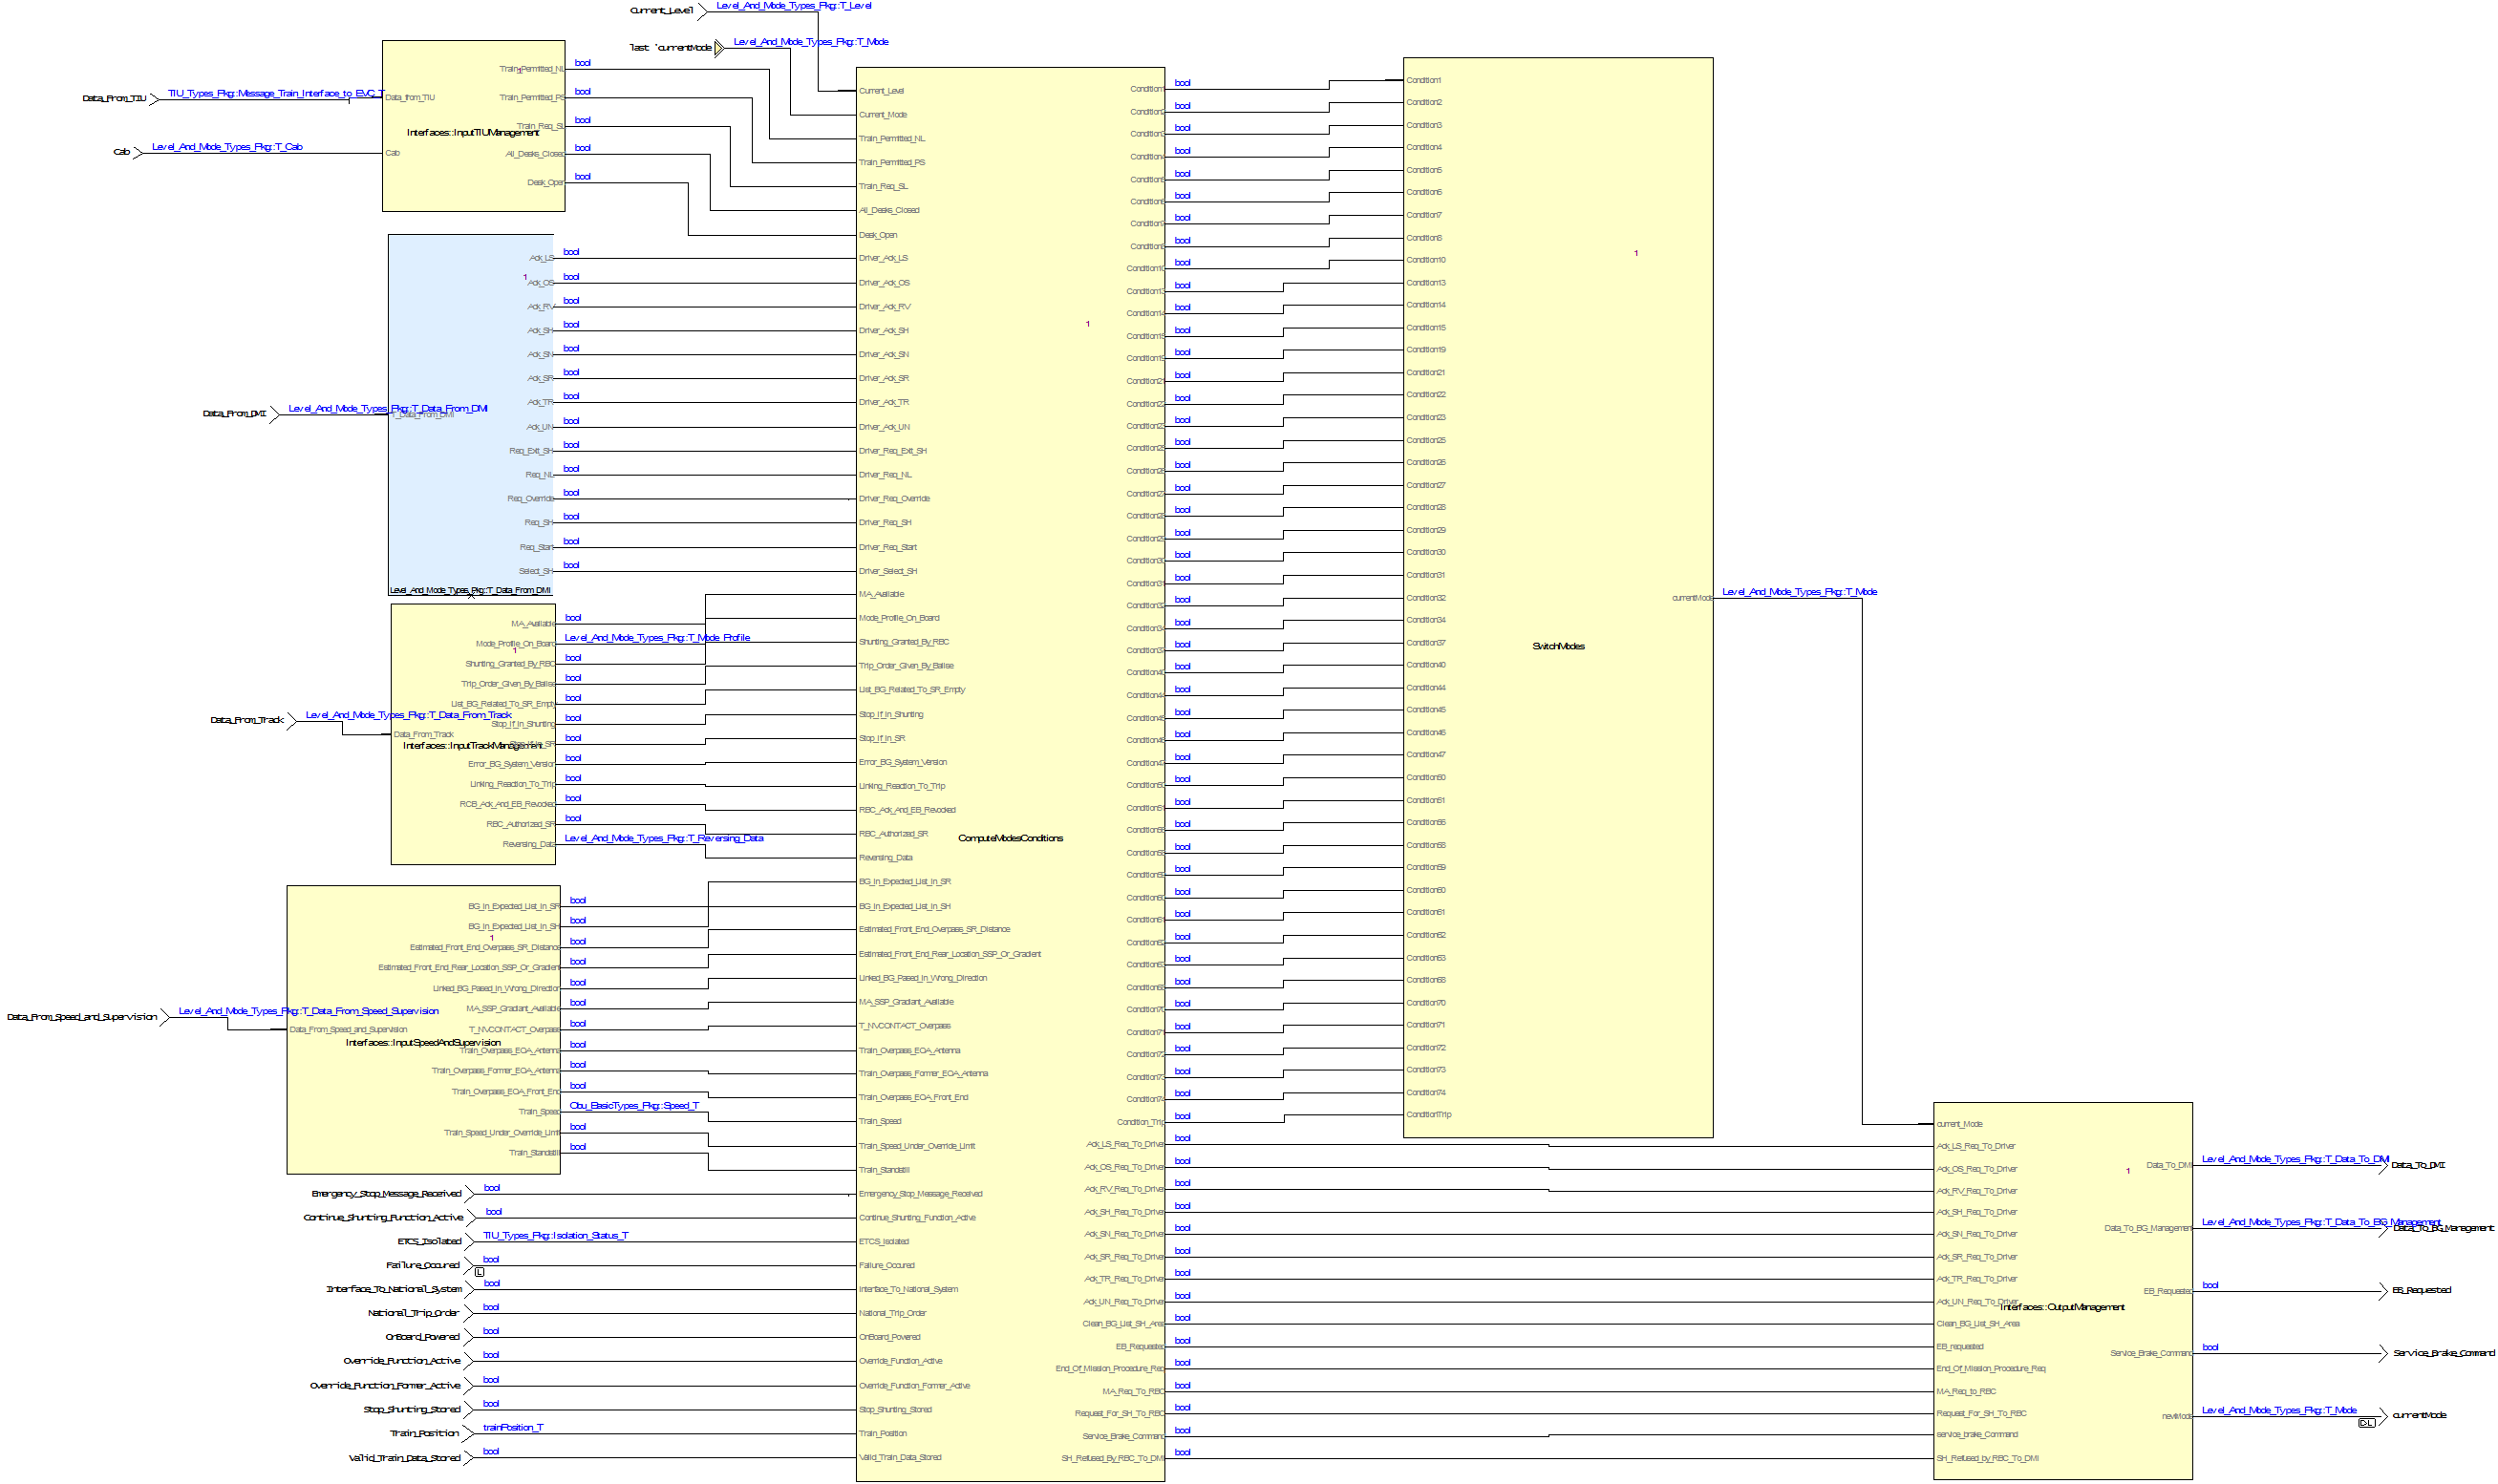
\includegraphics[scale=0.3]{images/ManageModes.png}
\caption{Modes subfubction architecture}
\end{figure}
\end{landscape}

\paragraph{Reference to the Scade Model}
The Scade model is available on github:
\url{https://github.com/openETCS/modeling/tree/master/model/Scade/System/ObuFunctions/ManageLevelsAndModes/Modes}

%%%%%%%%%%%%%%%%%%%%%%%%%%%%%%%%%%%%%%%%%%%%%%%%%%%%


\subsubsection{Function Check and Provide Level and Mode}%Mainfunction receive track data. Name should be be defined and substituded by the designer of the function.
\paragraph{Reference to the SRS or other Requirements}
see \citep{subset-026} section 3.6.5

\paragraph{Short description of the functionality}
checks compatibility between mode and level and provides outputs

\paragraph{Interface}
\emph{To design}

\paragraph{Functional Design Description}
\emph{To design}

\paragraph{Reference to the Scade Model}
\emph{To design}
